\documentclass[11pt,a4paper]{article}
\usepackage[margin=2.2cm]{geometry}
\usepackage{amsmath,amssymb}
\usepackage{siunitx}
\usepackage{booktabs}
\usepackage{xcolor}
\usepackage{microtype}
\usepackage{enumitem}
\usepackage{tcolorbox}
\usepackage{graphicx}
\definecolor{ink}{HTML}{14231B}\definecolor{accent}{HTML}{0F3D2A}
\tcbuselibrary{skins}
\newtcolorbox{key}{colback=accent!6,colframe=accent,boxrule=0.6pt,arc=2pt,left=6pt,right=6pt,top=4pt,bottom=4pt}
\sisetup{per-mode=symbol,group-separator={\,}}
\setlength{\parindent}{0pt}\setlength{\parskip}{6pt}
\renewcommand{\arraystretch}{1.25}

\title{\textbf{Slide 9: the SPI link}\\\large The protocol to the ZedBoard}
\author{ADS7057 test board v3 \quad ---\quad study notes}\date{}
\begin{document}\maketitle\vspace{-1.2em}
\section{The wires}
\begin{center}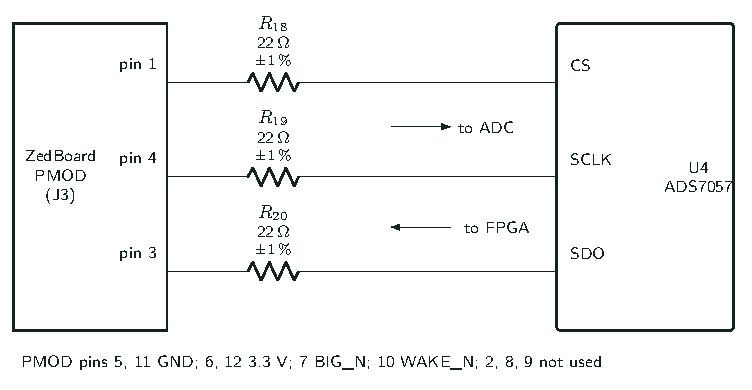
\includegraphics[width=0.9\textwidth]{s09_circuit.pdf}\end{center}
Three signal wires (CS, SCLK, SDO) and the two listener lines. There is no MOSI because the ADC only talks. The 22 Ω resistors sit at the ADC. With about \SI{10}{pF} of trace and pin (estimate), $\tau=22\,\Omega\times10\,\text{pF}=\SI{0.22}{ns}$ against a bit time of \SI{16.7}{ns} at \SI{60}{MHz}. They damp ringing and cost nothing in speed.

\section{One frame}
\begin{center}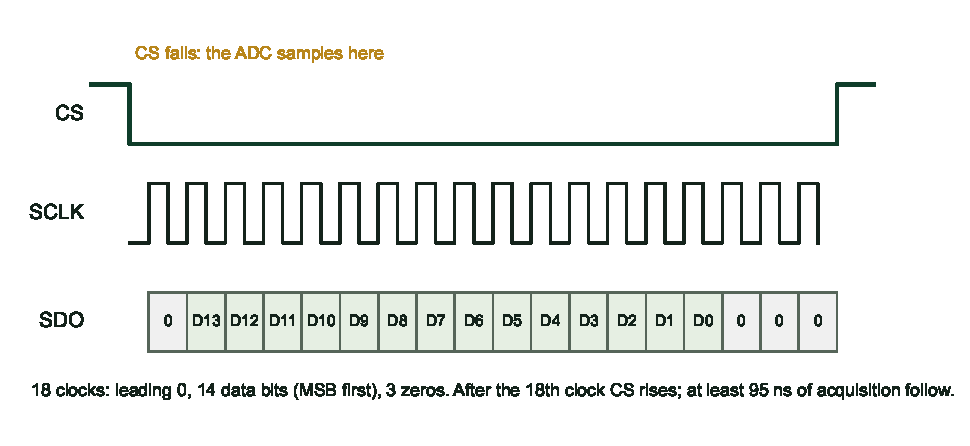
\includegraphics[width=0.85\textwidth]{s09_graph.pdf}\end{center}
CS falls and the ADC samples at that moment. The host sends 18 clocks. SDO shows a leading 0, the 14 data bits (MSB first) and three zeros. After the 18th clock the ADC converts nothing more. CS rises and the ADC acquires the next sample for at least \SI{95}{ns}.

\section{The data is one frame late}
The ADC sends the result of the previous conversion while it converts the current one. Frame 1 returns zeros, frame 2 returns sample 1, frame 3 returns sample 2. The FPGA must tag each word with the time of the \emph{previous} CS fall.

\section{Power-up}
The datasheet recommends an offset calibration. The first frame has 24 clocks, not 18. The ADC disconnects its input, corrects its offset and sends zeros. At \SI{20}{MHz} this takes $24/20\,\text{MHz}+95\,\text{ns}=\SI{1295}{ns}$. Repeat it when AVDD or the temperature changes a lot.

\section{How fast can it go}
One sample costs 18 clock periods plus the acquisition time:
\[
T_s=\frac{18}{f_\text{SCLK}}+95\,\text{ns},\qquad F_s=\frac1{T_s}.
\]
\begin{center}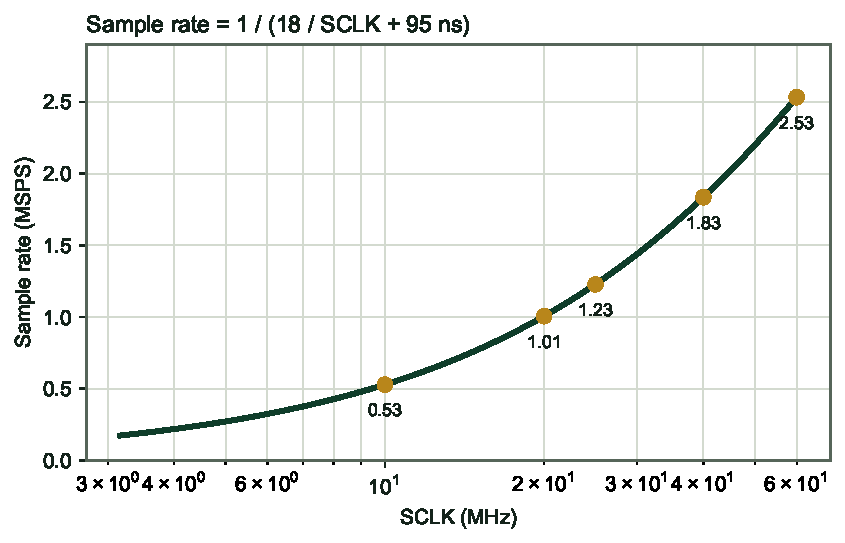
\includegraphics[width=0.6\textwidth]{s09_rate.pdf}\end{center}
\begin{center}\begin{tabular}{rrr}\toprule SCLK & one sample & rate\\\midrule
\SI{10}{MHz} & \SI{1895}{ns} & \SI{0.53}{MSPS}\\ \SI{20}{MHz} & \SI{995}{ns} & \SI{1.01}{MSPS}\\ \SI{25}{MHz} & \SI{815}{ns} & \SI{1.23}{MSPS}\\
\SI{40}{MHz} & \SI{545}{ns} & \SI{1.83}{MSPS}\\ \SI{60}{MHz} & \SI{395}{ns} & \SI{2.50}{MSPS}\\\bottomrule\end{tabular}\end{center}
The FPGA drives the ADC pins directly at 3.3 V (no level shifters on this board). Start at 10 to \SI{20}{MHz} and raise the clock after the first test. The sample rate sets the fold frequency of the anti-aliasing filter (slide 6): \SI{1.23}{MSPS} folds at \SI{615}{kHz}.
\begin{key}
On the 16-channel backplane (docs: \texttt{doc/backplane\_plan.md}) the link crosses level shifters, a ribbon and a buffer. The round trip adds about \SI{20}{ns} (estimate). Sample SDO one clock later than a plain SPI master would.
\end{key}
\end{document}
